\section{Theoretical Analysis of DIDA}
\label{sec:th_analysis_imitation}

The aim of this theoretical analysis is twofold. 
First, it provides bounds on the performance difference between that of the delayed policy and that of the undelayed policy. 
These bounds will depend on the assumption of the smoothness of the environment (see~\cref{{subsec:smooth_mdp}}). 
Second, studying these bounds will give us some insight on which undelayed expert might be more suited to be imitated in a delayed environment.  


\subsection{On the Comparison of Delayed and Undelayed Performance}
\label{subsec:compare_delayed_undelayed}

Before going straight to the theoretical results, it is useful to clarify one point. 
We would like to compare the value function of delayed and undelayed policies, yet, they do not share the same input space. 
Indeed, a delayed policy $\delayedpolicy$ has input space $\augmentedstatespace=\statespace\times\actionspace^\delay$ while the undelayed policy has input space $\statespace$. 
In the following, we will detail two ways of comparing these numbers that have been proposed in the literature.

\subsubsection{Comparison in Mildly Stochastic Markov Decision Processes}
One possibility to compare a delayed policy and an undelayed policy is proposed by \cite{walsh2009learning}. 
Their idea comes from the observation that, if a \gls{dmdp} derives from a deterministic \gls{mdp}, then they have identical optimal performance (up to the delay initialization shift of \Cref{subsec:delay_init}). 
This is easily understandable as, using the deterministic model of the environment to compute the current state, the agent can select the action that the undelayed policy recommends in this state. Obviously, the difficulty lies in learning the model of the \gls{mdp}.
To extend the comparison, \cite{walsh2009learning} consider what they refer to as a \textit{mildly stochastic} \gls{mdp}, that is, an \gls{mdp} where 
\begin{align*}
    \exists \epsilon \text{ s.t. } \forall (s,a)\in\statespace\times\actionspace, \exists s', p(s'\vert s,a)\geq 1-\epsilon.
\end{align*}
Since these \glspl{mdp} are only mildly stochastic, one could learn the optimal delayed policy for the deterministic approximation of the \gls{mdp} as described above. 
Doing so, and noting $\widehat{V}^{\pi}$ the value function of the undelayed policy in the deterministic approximation of the \gls{mdp}, one gets \cite[Theorem~3]{walsh2009learning}:
\begin{align*}
    \lVert \widehat{V}^{\pi}-{V}^{\pi}\rVert_{\infty}\leq \frac{\gamma\epsilon \maximumreward}{(1-\gamma)^2},
\end{align*}
where ${V}^{\pi}$ is the value function of the same policy $\pi$ but in the undelayed \gls{mdp}.
Note that these two value functions have $\statespace$ as input space. 
Another notable observation is the quadratic dependence on the effective time horizon $\textstyle\frac{1}{1-\gamma}$.
The assumption of mild stochasticity is quite strong and we will provide results for weaker assumptions.

\subsubsection{Comparison Under Belief Distribution}
Another approach that has the advantage of being applicable to any \gls{mdp} is that of \cite{agarwal2021blind}. 
For a given augmented state $x\in\augmentedstatespace$, the authors compare the value function of the delayed policy $V^{\delayedpolicy}(x)$ to the expected value function of an undelayed policy under the belief given $x$, $\textstyle\expectedvalue_{s\sim \augmentedbelief(\cdot\vert x)}[V^{\pi}(s)]$.
The authors propose learning a delayed policy that selects an action that maximises the expected undelayed policy's Q-function under the belief distribution. 
Provided that the action space is of finite cardinal $\cardinal{\actionspace}$, the delayed policy $\delayedpolicy$ has the following guarantee with respect to the optimal policy $\optimalpolicy$ \cite[Theorem~1]{agarwal2021blind}:
\begin{align*}
    V^\delayedpolicy(x) \ge \expectedvalue_{s\sim \augmentedbelief(\cdot\vert x)}[V^{\optimalpolicy}(s)] - \frac{\maximumreward}{(1-\gamma)^2}\left(1-\frac{1}{\cardinal{\actionspace}}\right)
\end{align*}
Note again the quadratic dependence on the effective time horizon.
We will compare the same quantities in our analysis while adding an assumption on the smoothness of the underlying \gls{mdp}. 




\subsection{Upper Bound on the Performance Loss  for Constant Delays}
\label{subsec:imitation_upper_bound}
In the remainder of this theoretical section, we assume that the underlying \gls{mdp} is smooth. To be more specific, we will need that the \gls{mdp} is  $(L_P,L_r)$-LC (see \Cref{def:lip_mdp}) and that the expert's undelayed policy is $L_\pi$-LC (see \Cref{def:lip_policy}). 
Furthermore, we will need its Q-function to be $L_Q$-LC\footnote{In some cases, this can be implied by the first two assumptions, see \Cref{th:lip_Q_function}.}.
These smoothness guarantees have the advantage of setting aside pathological examples such as the one of \Cref{pp:counter_example_belief_based}. 
However, the setting remains realistic, as many physical systems are Lipschitz. 

To provide our main result on an upper bound, we first derive an adaptation of the performance difference lemma~\cite[Lemma~6.1]{kakade2002approximately} to the delayed case. 
This result alone may be useful in the delayed literature. 
The result had been independently derived for integer delays in \cite[Equation~32]{agarwal2021blind} but we provide a more general version that applies to delay $\delay\in\realnumbers[\ge0]$.
In the following, we note $\discountedstateoccupancydistribution[x][\delayedpolicy]$ the discounted state occupancy distribution over the augmented state space $\augmentedstatespace$ for some delayed policy $\delayedpolicy$ starting from the augmented state $x$. 


\begin{lemma}
[Delayed Performance Difference Lemma]
\label{lem:perf_diff_lem}
    For some $\delay\in\realnumbers[\ge0]$, let $\pi$ be an undelayed policy and $\delayedpolicy$ be a $\delay$-delayed policy on the same underlying \gls{mdp} $\markovdecisionprocess$. 
    Then, $\forall x\in\mathcal{X}$,
    \begin{align*}
        \expectedvalue_{s\sim \augmentedbelief(\cdot\vert x)}[V^{\pi}(s)] - V^{\delayedpolicy}(x) 
        = \frac{1}{1-\gamma}
        \quad\expectedvalue_{x'\sim \delayeddiscountedstateoccupancydistribution[x][\delayedpolicy]} \left[ \expectedvalue_{s\sim \augmentedbelief(\cdot\vert x')}[V^{\pi}(s)] -  \expectedvalue_{\substack{s\sim \augmentedbelief(\cdot\vert x')\\a\sim \delayedpolicy(\cdot\vert x')}}[Q^{\pi}(s,a)] \right].
    \end{align*}
\end{lemma}
\begin{proof}
    Let us first demonstrate the result for an integer delay.
    
    \noindent\textbf{Integer delay.}\indent  Consider $\delay\in\naturalnumbers$, $x\in\augmentedstatespace$ and let
    \begin{align*}
        I(x)=\expectedvalue_{s\sim \augmentedbelief(\cdot\vert x)}[V^{\pi}(s)] - V^{\delayedpolicy}(x).
    \end{align*}
    By adding and subtracting the same quantity to $I$, we get:
    \begin{align*}
        I(x)
        &= \underbrace{\expectedvalue_{s\sim \augmentedbelief(\cdot\vert x)}[V^{\pi}(s)] - \expectedvalue_{\substack{s\sim \augmentedbelief(\cdot\vert x)\\a\sim \delayedpolicy(\cdot\vert x)}}\left[r(s,a) + \gamma \expectedvalue_{s'\sim p(\cdot\vert s,a)}[V^{\pi}(s')]\right]}_{\eqcolon A}
        \\
        &\quad + \underbrace{\expectedvalue_{\substack{s\sim \augmentedbelief(\cdot\vert x)\\a\sim \delayedpolicy(\cdot\vert x)}}\left[r(s,a) + \gamma \expectedvalue_{s'\sim p(\cdot\vert s,a)}[V^{\pi}(s')]\right] - V^{\delayedpolicy}(x)}_{\eqcolon B}.
    \end{align*}
    We then analyse each term of the above equation. First,
    \begin{align*}
        A = \expectedvalue_{s\sim \augmentedbelief(\cdot\vert x)}[V^{\pi}(s)] - \expectedvalue_{\substack{s\sim \augmentedbelief(\cdot\vert x)\\a\sim \delayedpolicy(\cdot\vert x)}}\left[Q^{\pi}(s,a)\right].
    \end{align*}
    Second, since $V^{\delayedpolicy}(x) = \expectedvalue_{\substack{s\sim \augmentedbelief(\cdot\vert x)\\a\sim \delayedpolicy(\cdot\vert x)}}\left[r(s,a)\right]+ \gamma \expectedvalue_{\substack{x'\sim \augmentedtransitionfunction(\cdot\vert x,a)\\a\sim \delayedpolicy(\cdot\vert x)}}[V^{\delayedpolicy}(x')]$, then,
    \begin{align*}
        B &= \gamma\expectedvalue_{\substack{s\sim \augmentedbelief(\cdot\vert x)\\a\sim \delayedpolicy(\cdot\vert x)}}\left[ \expectedvalue_{s'\sim p(\cdot\vert s,a)}[V^{\pi}(s')]\right] - \gamma \expectedvalue_{\substack{x'\sim \augmentedtransitionfunction(\cdot\vert x,a)\\a\sim \delayedpolicy(\cdot\vert x)}}[V^{\delayedpolicy}(x')].
    \end{align*}
    Note that,
    \begin{align}
    \label{eq:perf_diff_lem_equiv_belief}
        \int_{\statespace} \augmentedbelief(s\vert x)p(s'\vert s,a)\de s = \int_{\augmentedstatespace}\augmentedtransitionfunction(x'\vert x,a)\augmentedbelief(s'\vert x')\de x'.
    \end{align} 
    This means that, given the current augmented state $x$ and some action $a$, the probability that the next unobserved current state is $s'$ can be obtained in two ways. Either conditioning first on the current unobserved state $s$ or on the next augmented state $x'$.
    This yields,
    \begin{align*}
        B &= \gamma \expectedvalue_{\substack{x'\sim \augmentedtransitionfunction(\cdot\vert x,a)\\a\sim \delayedpolicy(\cdot\vert x)}}\left[\expectedvalue_{s\sim \augmentedbelief(\cdot\vert x')}[V^{\pi}(s')] - V^{\delayedpolicy}(x') \right]
        \\
        &= \gamma \expectedvalue_{\substack{x'\sim \augmentedtransitionfunction(\cdot\vert x,a)\\a\sim \delayedpolicy(\cdot\vert x)}}\left[I(x')\right],
    \end{align*}
    by recognising the quantity $I$. We now proceed by iterating this result as in the original lemma:
    \begin{align}
        I(x) &= \sum_{t=0}^\infty \gamma^t \expectedvalue_{\substack{x_{t+1}\sim \augmentedtransitionfunction(\cdot\vert x_t,a_t)\\a_t\sim \delayedpolicy(\cdot\vert x_t)}}\left[\left. \expectedvalue_{s\sim \augmentedbelief(\cdot\vert x_t)}[V^{\pi}(s)] - \expectedvalue_{\substack{s\sim \augmentedbelief(\cdot\vert x_t)\\a\sim \delayedpolicy(\cdot\vert x_t)}}[Q^{\pi}(s,a)] \right\vert x_0=x \right]\nonumber
        \\
        &= \frac{1}{1-\gamma}\expectedvalue_{x'\sim \delayeddiscountedstateoccupancydistribution[x][\delayedpolicy]}\left[ \expectedvalue_{s\sim \augmentedbelief(\cdot\vert x')}[V^{\pi}(s)] - \expectedvalue_{\substack{s\sim \augmentedbelief(\cdot\vert x')\\a\sim \delayedpolicy(\cdot\vert x')}}[Q^{\pi}(s,a)] \right],\label{eq:state_distrib_reco}
    \end{align}
    where \Cref{eq:state_distrib_reco} follows by the definition of the discounted augmented state occupancy distribution for policy $\delayedpolicy$ (see \Cref{def:discounted_state_distrib}). 
    Hence, the result for $\delay\in\naturalnumbers$.
    
    \noindent\textbf{Non-integer delay.}\indent For the sake of clarity of the proof, we assume $\delay\in(0,1)$ but the general result for $\delay\in\realnumbers[\ge0]$ easily derives from it.
    Note now that the belief is defined as in \Cref{subsec:non_int_delays}.
    The previous proof for integer delays can be applied without complications to non-integer delays. 
    The only step which might not easily follow is \Cref{eq:perf_diff_lem_equiv_belief}.
    Therefore, we detail this step below. 
    For $x_t=(s_t,a_{t-1}), x_{t+1}=(s_{t+1},a_t)\in\augmentedstatespace$,
    \begin{align}
        &\int_{\statespace} \augmentedbelief(s_{t+\delay}\vert x_t)p(s_{t+1+\delay}\vert s_{t+\delay},a)\de s_{t+\delay}\nonumber
        \\
        &\qquad=\int_{\statespace} \augmentedbelief(s_{t+\delay}\vert x_t) \int_{\statespace}  \augmentedbelief(s_{t+1+\delay}\vert s_{t+1},a) b_{1-\delay}(s_{t+1}\vert s_{t+\delay},a)\de s_{t+1}\de s_{t+\delay} \label{eq:use_def_p_non_int}
        \\
        &\qquad= \int_{\statespace} \augmentedbelief(s_{t+1+\delay}\vert s_{t+1},a)\int_{\statespace} \augmentedbelief(s_{t+\delay}\vert x_t)b_{1-\delay}(s_{t+1}\vert s_{t+\delay},a)\de s_{t+\delay}\de s_{t+1} \nonumber
        \\
        &\qquad= \int_{\statespace} \augmentedbelief(s_{t+1+\delay}\vert s_{t+1},a)\int_{\statespace} \augmentedbelief(s_{t+\delay}\vert s_t,a_{t-1})b_{1-\delay}(s_{t+1}\vert s_{t+\delay},a)\de s_{t+\delay}\de s_{t+1} \nonumber
        \\
        &\qquad= \int_{\actionspace} \int_{\statespace} \augmentedbelief(s_{t+1+\delay}\vert s_{t+1},a_{t}) \delta_{a}(a_{t})\nonumber
        \\
        &\qquad\quad\int_{\statespace} \augmentedbelief(s_{t+\delay}\vert s_t,a_{t-1}) b_{1-\delay}(s_{t+1}\vert s_{t+\delay},a)\de s_{t+\delay}\de s_{t+1}\de a_{t}\nonumber
        \\
        &\qquad= \int_\augmentedstatespace \augmentedbelief(s_{t+1+\delay}\vert x_{t+1})\tilde p(x_{t+1}\vert x_t, a)\de x_{t+1}\label{eq:def_aug_mdp_p_non_int}.
    \end{align}
    \Cref{eq:use_def_p_non_int} follows from the definition of $p$ in \Cref{eq:def_p_non_int} and \Cref{eq:def_aug_mdp_p_non_int} by recognising the transition in the augmented \gls{mdp}.
\end{proof}


We are now ready to state the main result of this chapter. 
This result is valuable not only for DIDA but for any policy that satisfies \Cref{eq:belief_pol}.
The smoothness of the \glspl{dmdp} is a key ingredient of the proof.

\begin{thm}
\label{th:perf_diff_bound}
    Let $\markovdecisionprocess$ be an $(L_P,L_r)$-LC \gls{mdp} and $\pi$ a $L_\pi$-LC undelayed policy. Assume also that $Q^{\pi}$ is $L_Q$-L.C.\footnote{The proof only requires the Lipschitzness of $Q^{\pi}$ in the second argument.}.
    Let $\delay\in\realnumbers[\ge0]$ and consider $\delayedpolicy$, a $\delay$-delayed policy that satisfies \Cref{eq:belief_pol}.
    Then, $\forall x\in\mathcal{X}$,
    \begin{align*}
        \expectedvalue_{s\sim \augmentedbelief(\cdot\vert x)}&[V^{\pi}(s)] - V^{\delayedpolicy}(x) \leq \frac{L_Q L_\pi}{1-\gamma} \sigma_b^x,
    \end{align*}
    where 
    \begin{align*}
        \sigma_b^x = \expectedvalue_{\substack{x'\sim \delayeddiscountedstateoccupancydistribution[x][\delayedpolicy]\\ s,s'\sim \augmentedbelief(\cdot\vert x')}}\left[ \distance_{\statespace}(s,s') \right].
    \end{align*}
\end{thm}
\begin{proof}
    For this proof, there is no need to separate integer and non-integer delays. 
    Let $\delay\in\realnumbers[\ge0]$. From \Cref{lem:perf_diff_lem}, for some $x \in \augmentedstatespace$,
    \begin{align*}
        \expectedvalue_{s\sim \augmentedbelief(\cdot\vert x)}&[V^{\pi}(s)] - V^{\delayedpolicy}(x) 
        = \frac{1}{1-\gamma} \expectedvalue_{x'\sim \delayeddiscountedstateoccupancydistribution[x][\delayedpolicy]} \bigg[\underbrace{ \expectedvalue_{s\sim \augmentedbelief(\cdot\vert x')}[V^{\pi}(s)] -  \expectedvalue_{\substack{s\sim \augmentedbelief(\cdot\vert x')\\a\sim \delayedpolicy(\cdot\vert x')}}[Q^{\pi}(s,a)]}_{A(x')} \bigg].
    \end{align*}
    Let us focus on the term $A(x')$. We have,
    \begin{align}
        A(x')
        &= \expectedvalue_{s\sim \augmentedbelief(\cdot\vert x')}\left[\expectedvalue_{\substack{a_1\sim\pi(\cdot\vert s) \\a_2\sim \delayedpolicy(\cdot\vert x')}}\left[ Q^{\pi}(s,a_1) -  Q^{\pi}(s,a_2) \right]\right]\nonumber
        \\
        &\leq L_Q \expectedvalue_{s\sim \augmentedbelief(\cdot\vert x')} \left[ \wassersteindistance(\pi(\cdot\vert s)
        \Vert \delayedpolicy(\cdot\vert x') ) \right],\label{eq:partial_res_v}
    \end{align}
    where the result follows from the application of \Cref{pp:expected_q_bound}.
    The last step is to upper bound 
    $\expectedvalue_{s\sim \augmentedbelief(\cdot\vert x')} \left[ \wassersteindistance(\pi(\cdot\vert s) \Vert \delayedpolicy(\cdot\vert x') ) \right]$ using
    $\sigma_b^x$. Thus,
    \begin{align}
         \wassersteindistance(\pi(\cdot\vert s) \Vert \delayedpolicy(\cdot\vert x') ) 
        &= \sup_{\left\Vert f\right\Vert_L\leq 1}\left\vert\int_{\actionspace} f(a)(\pi(a\vert s)-\delayedpolicy(a\vert x')) \de a\right\vert \nonumber
        \\
        &= \sup_{\left\Vert f\right\Vert_L\leq 1}\left\vert\int_{\actionspace} f(a)(\pi(a\vert s)-\int_{\statespace}\pi(a\vert s')\augmentedbelief(s'\vert x')\de s') \de a\right\vert \label{eq:def_pidel}
        \\
        &\leq  \int_{\statespace} \augmentedbelief(s'\vert x') \sup_{\left\Vert f\right\Vert_L\leq 1}\left\vert\int_{\actionspace} f(a)(\pi(a\vert s)-\pi(a\vert s')) \de a \right\vert \de s' \label{eq:fub_ton_sigma}
        \\
        &\leq \int_{\statespace} \augmentedbelief(s'\vert x') \wassersteindistance(\pi(\cdot\vert s) \Vert \pi(\cdot\vert s') ) \de s'\nonumber
        \\
        &\leq L_\pi \int_{\statespace} \augmentedbelief(s'\vert x')  \distance_{\statespace}(s,s') \de s'
        \label{eq:lip_expert_pol}
        ,
    \end{align}
    where \Cref{eq:def_pidel} follows from \Cref{eq:belief_pol}, \Cref{eq:fub_ton_sigma} by the Fubini-Tonelli theorem  and \Cref{eq:lip_expert_pol} by Lipschitzness of $\pi$.
    It now suffices to reinject this result into \Cref{eq:partial_res_v} to conclude.
\end{proof}

To allow more practical interpretations of this result, we provide two ways to further bound the uncommon term $\sigma_b^x$, each introducing a new assumption.  
The first result assumes the time-Lipschitzness of the \gls{mdp} (see \Cref{def:time_lip}).

\begin{coroll}
\label{cor:perf_diff_bound_tlc}
    If the assumptions of \Cref{th:perf_diff_bound} hold and, in addition, the \gls{mdp} is $L_T$-TLC, then, $\forall x\in\mathcal{X}$,
    \begin{align*}
        \expectedvalue_{s\sim \augmentedbelief(\cdot\vert x)}&[V^{\pi}(s)] - V^{\delayedpolicy}(x) \leq \frac{2 \delay L_T L_Q L_\pi}{1-\gamma}.
    \end{align*}
\end{coroll}
\begin{proof}
    Applying \Cref{lem:bound_sigma_tlc} to \Cref{th:perf_diff_bound} provides the result.
\end{proof}

This result clearly shows that the bound on the performance difference depends linearly on the delay. 
One critical limitation to this bound is that it does not go to 0 as the \gls{mdp} becomes deterministic. In fact, as we have seen in \Cref{subsec:compare_delayed_undelayed}, the optimal delayed return should match the undelayed one in this case.
The second corollary to \Cref{th:perf_diff_bound} that we are now presenting does not have this limitation. 

\begin{coroll}
\label{cor:perf_diff_bound_eucl}
    If the assumptions of \Cref{th:perf_diff_bound} hold and, in addition, $\statespace\subseteq\realnumbers^n$ is equipped with the Euclidean norm, then, $\forall x\in\mathcal{X}$,
    \begin{align*}
        \expectedvalue_{s\sim \augmentedbelief(\cdot\vert x)}[V^{\pi}(s)] - V^{\delayedpolicy}(x) \leq
        \frac{\sqrt{2} L_Q L_\pi}{1-\gamma}
        \expectedvalue_{x'\sim \delayeddiscountedstateoccupancydistribution[x][\delayedpolicy]}\left[\sqrt{ \variance_{s\sim \augmentedbelief(\cdot\vert x')}(s\vert x')}\right].
    \end{align*}
\end{coroll}
\begin{proof}
    Applying \Cref{lem:bound_sigma_eucl} to \Cref{th:perf_diff_bound} provides the result.
\end{proof}

To appreciate the quality of these bounds, we now provide a result on a lower bound of the performance difference. 


\subsection{Lower Bound on the Performance Loss for Constant Delays}
In this subsection, we add significance to \Cref{cor:perf_diff_bound_eucl} by showing that it matches a lower bound up to a constant term when the expert's undelayed policy is optimal and under the same smoothness assumptions.

\begin{thm}
\label{th:lb_tight}
Let $L_\pi>0$, $L_{Q}>0$, and $\delay\in\realnumbers[\ge0]$. 
Then there exists an \gls{mdp} with an optimal $L_\pi$-LC policy $\optimalpolicy$ such that its value function is $L_{Q}$-LC in the second argument, but for any $\delay$-delayed policy $\delayedpolicy$, and $x\in\augmentedstatespace$
    \begin{align*}
        \expectedvalue_{s\sim \augmentedbelief(\cdot\vert x)}[\optimalstatevaluefunction(s)] - V^{\delayedpolicy}(x) &\geq
        \frac{\sqrt 2}{\sqrt \pi}\frac{ L_{Q}L_\pi}{1-\gamma}
        \expectedvalue_{x'\sim \delayeddiscountedstateoccupancydistribution[x][\delayedpolicy]}\left[\sqrt{ \variance_{s\sim \augmentedbelief(\cdot|x')}(s|x')}\right],
    \end{align*}
    where $\optimalstatevaluefunction$ is the value function of the optimal undelayed policy.
\end{thm}
\begin{proof}
    For given values of $L_\pi>0$, $L_{Q}>0$ and $\delay\in\realnumbers[\ge0]$, we design an \gls{mdp} $\markovdecisionprocess=(\statespace,\actionspace, \transitionfunction, \rewardfunction, \initialstatedistribution)$ such that: $\statespace=\realnumbers$; $\actionspace=\realnumbers$; its transition function is 
    \begin{align*}
        \transitionfunction(s'\vert s,a)=\mathcal N\left(s';\; s+\frac{a}{L_\pi},\sigma^2\right),
    \end{align*} 
    that is, $s'=s+\frac{a}{L_\pi}+\varepsilon$, where $\varepsilon \sim \mathcal N (0,\sigma^2)$;
    its reward function is
    \begin{align*}
        \expectedrewardfunction(s,a)=\expectedvalue[\rewardfunction(s,a)] = -L_r\left\vert s+\frac{a}{L_\pi}\right\vert,
    \end{align*}
    where $L_r:=L_Q L_\pi$.
    We have used $L_Q$ in the definition of $\expectedrewardfunction$ since we will show later that this is exactly the Lipschitz constant of $\optimalstateactionvaluefunction$.
    Note that $\forall (s,a)\in\statespace\times\actionspace,\;r(s,a)\le0$, but the policy $\optimalpolicy(a\vert s)=\delta_{-L_\pi s}(a)$ gets a reward of $0$ for any pair $(s,a)$. 
    This implies that $\optimalstatevaluefunction=0$ everywhere.
    
    We now prove that the Q-function is Lipschitz,
    \begin{align*}
        \optimalstateactionvaluefunction(s,a)&=-L_r\left\vert s+\frac{a}{L_\pi}\right\vert + \gamma \int_{\realnumbers} \optimalstatevaluefunction(s')\ p(s'\vert s,a)\de s'
        \\
        &= -L_r\left\vert s+\frac{a}{L_\pi}\right\vert
        \\
        &=-L_{Q}\left\vert L_\pi s+a\right\vert.
    \end{align*}
    Hence, $\optimalstateactionvaluefunction$ is $L_Q$-LC in the second argument.
    
    We now study the case of a $\delay$-delayed policy $\delayedpolicy$.
    For a given time step $t$, the unobserved current state is
    \begin{align*}
        s_t=\underbrace{s_{t-\delay}+\sum_{\tau=t-\delay}^{t-1} \frac{a_\tau}{L_\pi}}_{\eqqcolon \phi(x_t)}+\underbrace{\sum_{\tau=t-\delay}^{t-1} \varepsilon_\tau}_{\eqqcolon\epsilon}.
    \end{align*}
    We have defined two quantities above. The first, $\phi(x_t)$, is a deterministic function of an augmented state $x_t\in\augmentedstatespace$. 
    The second, $\epsilon$, is a random variable with distribution $\mathcal N(0,\delay\sigma^2)$.
    Using these quantities, we can define the augmented reward as,
    \begin{align*}
        \augmentedexpectedrewardfunction (x_t,a)
        &= -L_r\expectedvalue\left[\Big\vert s_t+\frac{a}{L_\pi}\Big\vert\right]
        \\
        &=-L_r\expectedvalue\left[\Big\vert\phi(x_t)+\frac{a}{L_\pi}+\epsilon\Big\vert\right].
    \end{align*}
    The reward is therefore proportional to the function $f:a\mapsto\expectedvalue\left[\left\vert \mathcal N(g(a),\delay\sigma)\right\vert\right]$ for $\textstyle g(a)=\phi(x_t)+\frac{a}{L_\pi}$. The minimum of $f$ is attained for $g(a)=0$ and corresponds to the mean of a half-normal distribution, that is $\textstyle\min_{a\in\realnumbers}f(a)=\frac{\sigma\sqrt{2\delay}}{\sqrt{\pi}}$ and therefore,
    \begin{align*}
        \augmentedexpectedrewardfunction (x_t,a)
        &\le -{L_r}\frac{\sqrt {2\delay}}{\sqrt \pi}\sigma.
    \end{align*}
    Thus,
    \begin{align*}
        V^{\delayedpolicy}(x)
        &= \expectedvalue_{\substack{x_{t+1}\sim\augmentedtransitionfunction(\cdot\vert x_t,a_t)\\a_t\sim\delayedpolicy(\cdot\vert s_t)}} \left[\left.\sum_{t=0}^\infty \gamma^t \augmentedexpectedrewardfunction(x_t,a_t)\right\vert x_0=x\right]
        \\
        &\leq-\frac{L_r}{1-\gamma}\frac{\sqrt {2\delay}}{\sqrt \pi}\sigma
        \\
        &= -\frac{L_Q L_\pi}{1-\gamma}\frac{\sqrt {2}}{\sqrt \pi}\expectedvalue_{x'\sim \delayeddiscountedstateoccupancydistribution[x][\delayedpolicy]}\left[\sqrt{ \variance_{s\sim \augmentedbelief(\cdot|x')}(s|x')}\right],
    \end{align*}
    where, in the first inequality, we note that the variance is the same for any unobserved current state given the definition of $\markovdecisionprocess$. 
    In the last inequality,  we have replaced $L_r$ by $L_Q L_\pi$ and $\delay\sigma^2$ by the variance over the belief 
    $\mathbb Var_{s\sim b(\cdot\vert x)}(s\vert x)$.
    This inequality and the fact that $\optimalstatevaluefunction=0$ at any state conclude the proof.
\end{proof}

This result highlights that the coarser the expert policy, the weaker the guarantees. 

\subsection{Implications for Constant Delays}
We will now discuss the implications of the previous theoretical results. 
These bounds hold if the policy $\delayedpolicy$ has perfectly imitated the undelayed policy and satisfies \Cref{eq:belief_pol}. 
In practice, this might not be the case and is a first source of performance loss.
A second source of performance loss is that the undelayed policy itself might not be optimal and, although this does not impact the bounds, it lowers the final performance of the agent.

In particular, we point out two key trade-offs. 
First, a smoother expert might be sub-optimal in the undelayed environment, but it provides a much simpler imitation problem to the delayed policy according to \Cref{th:perf_diff_bound}. 
Second, a noisier policy might also be sub-optimal in the undelayed environment but, by providing examples of bad decisions and how to recover from them, it can simplify the imitation task~\cite{laskey2017dart}.



\subsection{Bounds on the Performance Loss for Stochastic Delays}
\label{subsec:stoch_delay_dida}
In this sub-section, we study the guarantees of DIDA when applied to stochastic integer delays. 
Action execution and state observation delays may not be equivalent in this case, depending on the stochasticity of the delay.
The equivalence has been shown only for special types of stochastic delays \cite[Result~2]{katsikopoulos2003markov} and in \cite{bouteiller2020reinforcement}.
In the latter result, the definition of the stochastic delay is similar to the definition that we will introduce below.
We consider a delayed state observation whose delay sequence $(\delay_t)_{t\ge0}$ is i.i.d. with discrete distribution $\zeta$, of support $[\![0,\delaymax]\!]$.
As an example, $\probability(\delay_t=k)= \zeta(k)$ is the probability that state $s_t$ is observed at time $s_{t+k}$. 
We note $\zeta(k\vert i)$ the probability that $\delay_t=k$ knowing that $\delay_t>i$.
We also assume that the delay is non-anonymous, that is, whenever a new observation is collected by the agent, the observation's original time step is known. 
This avoids credit assignment problems.

Within this framework, one can consider the following augmented state $x\in\widecheck{\augmentedstatespace}\coloneq\statespace\times\actionspace^{\delaymax}\times\naturalnumbers$:
\begin{align*}
    x = (s,a_1,\dots,a_\delaymax,n),
\end{align*}
where $(a_1,\dots,a_\delaymax)$ is the usual action buffer, $s$ is the most recent observed state and $n$ indicates the time difference between the time at which $s$ has been observed and the current time. 
Said alternatively, $n$ is the effective current delay. 
We assume that the augmented state is available to the agent, the delay is therefore contained in the information structure of the agent (see \Cref{subsec:control_theory}).
In the following, we will see that the fact that the delay is non-anonymous is key to the definition of this problem. 
Clearly, for $n<\delaymax$, some actions from the augmented state are useless, as a more recent state has been observed. 
This framework is reminiscent of the stochastic delay framework of \cite{bouteiller2020reinforcement}.

Next, we define the transition probability for this new process, which we note $\augmentedtransitionfunction$. 
For two augmented states $x = (s,a_1,\dots,a_\delaymax,n)$ and $x' = (s',a_1',\dots,a_\delaymax',n')$
\begin{align}
\label{stochastic_delay_transition}
    \augmentedtransitionfunction(x'\vert x,a) = \probability(O=n+1-n')  p^{n+1-n'}(s'\vert x,a)
\delta_a(a_{\delaymax}')\prod_{i=1}^{\delaymax-1}\delta_{a_{i+1}}(a_{i}').
\end{align}
Some new terms have been introduced in this equation.
First, the random variable $O$. 
It is the difference in the number of steps between the previous last observed state $s$ and the new last observed state $s'$.
One can compute its probability as:
\begin{align}
    \probability(O=k) &= \zeta(n-k+1\vert n-k)
    \nonumber\\
    &\qquad\cdot\left(1-\zeta(0)\right)\prod_{i=1}^{n-k} \left(1-\zeta(n-k+1-i\vert n-k-i)\right),\label{eq:observed}
\end{align}
where $\zeta(n-k+1\vert n-k)$ is the probability that the state $k$ steps after $s$ is observed, and the following terms in $(1-\zeta(\cdot))$ make sure that the more recent states are not observed. 
Note that $n'=n-k+1$.
Note also that the observation of states in between $s$ and $s'$ is irrelevant for the transition probability.
From this observation, $O$ can be considered as the number of observations at a given step.
A visual representation on how to interpret the random variable $O$ is given in \Cref{fig:random_delay}.
Second, the term $p^{n+1-n'}(s'\vert x,a)$ in \Cref{stochastic_delay_transition} is the $n+1-n'$-step transition in the underlying \gls{mdp} starting from $s$ and following the sequence of actions in $x$ and then $a$, for as many steps as needed.

\begin{figure}[t]
    \centering
    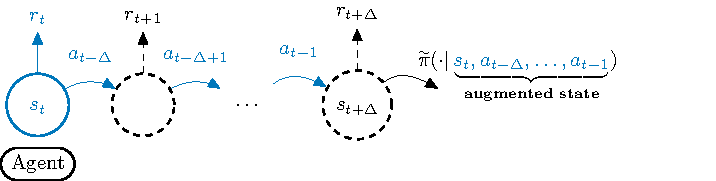
\includegraphics[bylabel=randomdelay]{img/thesis_plots.pdf}
    \caption{Example of a stochastic delay where
    at time $t$ the delay was $n$ and at time $t+1$ the delay will be $n'=n-1$.
    This implies that the agent has observed 2 new states.
    The random variable for the number of observations between steps, $O$, has a probability defined as the product of the probabilities as in \Cref{eq:observed}.
    Note that the probability to observe or not the state with index $t-n+1$ is irrelevant because a more recent one has been observed.}
    \label{fig:random_delay}
\end{figure}


One can define the reward of this process as follows,
\begin{align*}
    \augmentedexpectedrewardfunction(x,a) = \sum_{k=0}^{n}\probability(O=k)\sum_{i=0}^{k-1} \gamma^i\expectedvalue_{s_i\sim p^i(s_i\vert x,a)}[r(s_i,a_i)].
\end{align*}
This reward basically sums up all the rewards for the newly observed steps. 
This definition assumes that whenever a state is observed, all the intermediate states that had not been observed yet will be observed contemporaneously.

Clearly, the process involving the augmented state defines an \gls{mdp} and proves the following proposition.

\begin{prop}
\label{pp:stoch_dmdp_is_mdp}
    The \gls{dmdp} with i.i.d. delays $(\delay_t)_{t\ge0}$ with discrete distribution $\zeta$ as defined above can be cast into an \gls{mdp} by augmenting the state with a buffer of the last $\delaymax$ actions and the effective current delay.
\end{prop}
This proposition has also been found in \cite{bouteiller2020reinforcement} for a more general setting of both state observation and action execution delay.  
We note that including action execution delay poses the problem of potentially having no action executed at a given time step or multiple actions executed at a given time step. 
In these cases, the behaviour of the environment must be defined.

We will now consider applying a policy $\delayedpolicy$ learnt by DIDA in this framework to study the impact of wrongly assuming a constant delay when the true environment is stochastically delayed. 
Note that the constant $\delay$-delayed \gls{dmdp} where DIDA has been trained can be seen as an example of the above process where the whole weight of the $\zeta$ distribution has been placed at $\delay$.
In this case, for $x = (s,a_1,\dots,a_\delaymax,n)$, we consider that $\delayedpolicy(\cdot\vert x) = \delayedpolicy(\cdot\vert s,a_{\delaymax-\delay+1},\dots,a_\delaymax)$. 
In fact, DIDA considers the state $s$ as being $\delay$-delayed and is blind to $n$.
We compare DIDA with a policy $\widecheck{\pi}$ with the following definition:
\begin{align}
    \widecheck{\pi}(a\vert x) = \int_{\statespace} \augmentedbelief[n](s\vert x) \pi(a\vert s) \de s.\label{eq:belief_pol_stoch}
\end{align}
This policy has a construction similar to that of DIDA but adapts to the value of $n$. 
In the following, we note $\widebar\delay$ the mean delay of the stochastically delayed process. It is defined as follows,
\begin{align*}
    \widebar\delay = \expectedvalue[n] =  \sum_{k=0}^{\delaymax}k\prod_{i=0}^{k-1}\probability(\delay_i>i)\probability(\delay_k=k)
\end{align*}


\begin{thm}
\label{thm:stoch_mdp_dida_bound}
    Consider a \gls{dmdp} with stochastic delay as previously defined and assume that the underlying \gls{mdp} is $L_T$-TLC.
    Consider the policy $\delayedpolicy$ learnt by DIDA for constant delay (\Cref{eq:belief_pol}) and the policy $\widecheck\pi$ (\Cref{eq:belief_pol_stoch}).
    Assume that the Q-function $Q^\delayedpolicy$ of $\delayedpolicy$ is $L_{\widetilde Q}$-LC in the second argument\footnote{This holds for example if $\gamma\max(L_P,1)\cdot(1+2L_\pi L_P)<1$. This result is obtained by application of \cite[Theorem~1]{rachelson2010locality} to the Lipschitz constant of a constantly delayed \gls{mdp} (\Cref{pp:lip_dmdp}) and the policy of DIDA (\Cref{pp:lip_dida_pol}).}. 
    Then the difference in performance between $\delayedpolicy$ and the policy $\widecheck\pi$ can be bounded as,
    \begin{align*}
        \lvert V^{\widecheck{\pi}}(x)- V^{\delayedpolicy}(x)\rvert \le \frac{L_{\widetilde Q} L_\pi L_T }{1-\gamma}(\widebar\delay+\delay).
    \end{align*}
\end{thm}
\begin{proof}
    From \Cref{pp:stoch_dmdp_is_mdp}, we know that the stochastically delayed \gls{dmdp} is an \gls{mdp}. Therefore, the regular performance difference lemma can be applied and yields, for $x\in\widecheck{\augmentedstatespace}$\footnote{Note that in this proof, we overwrite the notation $\delayeddiscountedstateoccupancydistribution[x][\delayedpolicy]$ that was defined for constantly delayed \gls{dmdp} over the space $\augmentedstatespace$ and use the space $\widecheck\augmentedstatespace$ as its domain instead.},
    \begin{align*}
        V^{\widecheck{\pi}}(x)- V^{\delayedpolicy}(x) 
        = \frac{1}{1-\gamma} \expectedvalue_{x'\sim \delayeddiscountedstateoccupancydistribution[x][\widecheck\pi]} \left[\underbrace{V^{\delayedpolicy}(x) -  \expectedvalue_{a\sim \widecheck\pi(\cdot\vert x')}[Q^{\delayedpolicy}(x,a)]}_{A(x')}\right].
    \end{align*}
    As in \Cref{th:perf_diff_bound}, we can derive the following bound by application of \Cref{pp:expected_q_bound}, where we note $x'=(s',a_1',\dots,a_\delaymax',n')$, 
    \begin{align}
        A(x') 
        &\leq L_{\widetilde Q} \wassersteindistance(\widecheck\pi(\cdot\vert x')
        \Vert \delayedpolicy(\cdot\vert x'))
        \nonumber\\
        &= L_{\widetilde Q} \sup_{\left\Vert f\right\Vert_L\leq 1}\left\vert\int_{\actionspace} f(a)(\widecheck\pi(a\vert x')-\delayedpolicy(a\vert x') \de a\right\vert 
        \nonumber\\
        &= L_{\widetilde Q} \sup_{\left\Vert f\right\Vert_L\leq 1}\left\vert\int_{\actionspace}\int_{\statespace} f(a)\pi(a\vert s)(\augmentedbelief[n'](s\vert x')-\augmentedbelief(s\vert x'))\de s  \de a\right\vert
        \nonumber\\
        &\leq L_{\widetilde Q} L_\pi \wassersteindistance(\augmentedbelief[n'](\cdot\vert x')
        \Vert \augmentedbelief(\cdot\vert x'))
        \nonumber\\
        &\leq L_{\widetilde Q} L_\pi L_T (n'+\delay),\label{eq:l_t_lip}
    \end{align}
    where we have set $\augmentedbelief(s\vert x')=\augmentedbelief(s\vert s',a_1',\dots,a_\delaymax')$. We have used the fact that the undelayed policy $\pi$ is $L_{\pi}$-LC and \Cref{eq:l_t_lip} follows easily by replicating the proof of \Cref{lem:bound_sigma_tlc}. 
    Therefore,
    \begin{align*}
        V^{\widecheck{\pi}}(x)- V^{\delayedpolicy}(x) 
        &\leq \frac{L_Q L_\pi L_T }{1-\gamma} \left(\delay +\expectedvalue_{x'\sim \delayeddiscountedstateoccupancydistribution[x][\widecheck\pi]}[n']\right)
        \\
        &= \frac{L_Q L_\pi L_T }{1-\gamma} \left(\delay +\widebar\delay\right),
    \end{align*}
    where the last equality holds by integrating out the terms of the augmented state but $n'$.
\end{proof}

Note the importance of the time Lipschitzness in the proof. 
Without this assumption, the dependence on $x'$ of $\wassersteindistance(\augmentedbelief[n'](\cdot\vert x')\Vert \augmentedbelief(\cdot\vert x'))$ remains, and it is not clear what its expectation under $\delayeddiscountedstateoccupancydistribution[x][\widecheck\pi]$ is.
There is indeed a non-obvious dependence between $n$ and the rest of the element in the augmented state. 
For example, it is possible that some states of $\statespace$ are visited more often when the delay is smaller. 
Note also that the assumption of \Cref{th:perf_diff_bound} of $\statespace\subseteq\realnumbers^n$ equipped with the Euclidean norm is of little help here since $\wassersteindistance(\augmentedbelief[n'](\cdot\vert x')\Vert \augmentedbelief(\cdot\vert x'))$  potentially compares trajectories of different length ($n'\neq\delay$).
The fact that DIDA is blind to the true delay in this framework constitutes a case of anonymous delay (see \Cref{subsec:anonymous_delay_related}). 
To the best of our knowledge, this is the first result on anonymous state observation delay in \gls{rl}.


